\chapter{Controle de Referências}

\hologo{BibTeX} é uma ferramenta e um formato de arquivos usados para descrever e processar listas de referência,       normalmente em documentos \LaTeX  . Na prática, o termo  é usado como termo geral para tratar de dois conjuntos distintos de aplicações associadas ao \LaTeX:
\begin{outline}
    \1 \hologo{BibTeX} e \hologo{biber}, programas que
    processam a informação bibliográfica de um documento \LaTeX\ e criam a bibliografia
    \1 natbib e biblatex, pacotes \LaTeX\ que formatam as citações e a bibliografia
    \2 natbib só funciona com \hologo{BibTeX}
    \2 biblatex funciona com ambos processadores
\end{outline}

%%CHECK 1

\section{O arquivo .bib}

O funcionamento básico do \hologo{BibTeX}  depende de um arquivo .bib, exemplificado no figura \ref{fig:bibfile}, que é uma base de dados contendo  referências contendo uma chave de citação. Essa base é construída em um arquivo texto comum, o que permite que seja manipulada tanto por programas específicos, quanto pelos autores diretamente. Ao longo do texto, o autor pode fazer citações a essas referências usando comandos como \lstinline|\cite{Xexeo2020}|. 

A interação entre o processador \LaTeX, o pacote escolhido e o processador de referências escolhido, também conhecido com \textit{backend engine}, trará para a versão a ser impressa as citações e a bibliografia no formato desejado. 

Como pode ser visto na figura \ref{fig:bibfile}, um arquivo .bib é compostos de entradas, como \lstinline|@book| que são, por sua vez, compostas de campos, obrigatórios ou opcionais, como \lstinline|author|. As entradas geram formatos específicos na bibliografia, de acordo com as normas utilizadas.

%THE BUG IS AFTER

\begin{lstlisting}[caption=Exemplo de arquivo .bib,label=fig:bibfile]
@book{sommerville:requirements,
author = {Sommerville, Ian and Sawyer, Pete},
title = {Requirements Engineering: A Good Practice Guide},
year = {1997},
isbn = {0471974447},
publisher = {John Wiley \& Sons, Inc.},
address = {USA},
edition = {1}
}

@article{therac25,
author       = {Nancy G. Levenson and Clark S. Turner},
title        = {An Investigation of the Therac-25 Accidentes},
journaltitle = {Computer},
date         = {1993-07},
volume       = {26},
number       = {7},
pages        = {18-41},
}
\end{lstlisting}


%THE BUG IS BEFORE

\subsection{Tipos de Entradas Mais Usados}

Os tipos de entradas mais usados são:
\begin{itemize}
    \item article
    \item inbook
    \item book
    \item incollection
    \item collection
    \item inproceedings
    \item proceedings
    \item report
    \item thesis
    \item online
    \item misc
\end{itemize}

%CHECKEND

\section{O Ecossistema BibTeX}


A figura \ref{fig:mundolatexport}\autocite{bibera2012}, descreve o ecossistema \hologo{BibTeX}. Ele é formado por pacotes que executam no processador \LaTeX , processadores para bibliografia, arquivos com bases de referência, programas que gerenciam esses arquivos (o que pode ser feito com editores de texto, no caso de arquivos .bib), e, possivelmente, outros programas que fazem transformações de arquivos. A figura mostra que há duas escolhas a serem feitas: o pacote \LaTeX\  a ser usado e o processador
a ser escolhido. 

\begin{figure}[hbt]
    \centering
    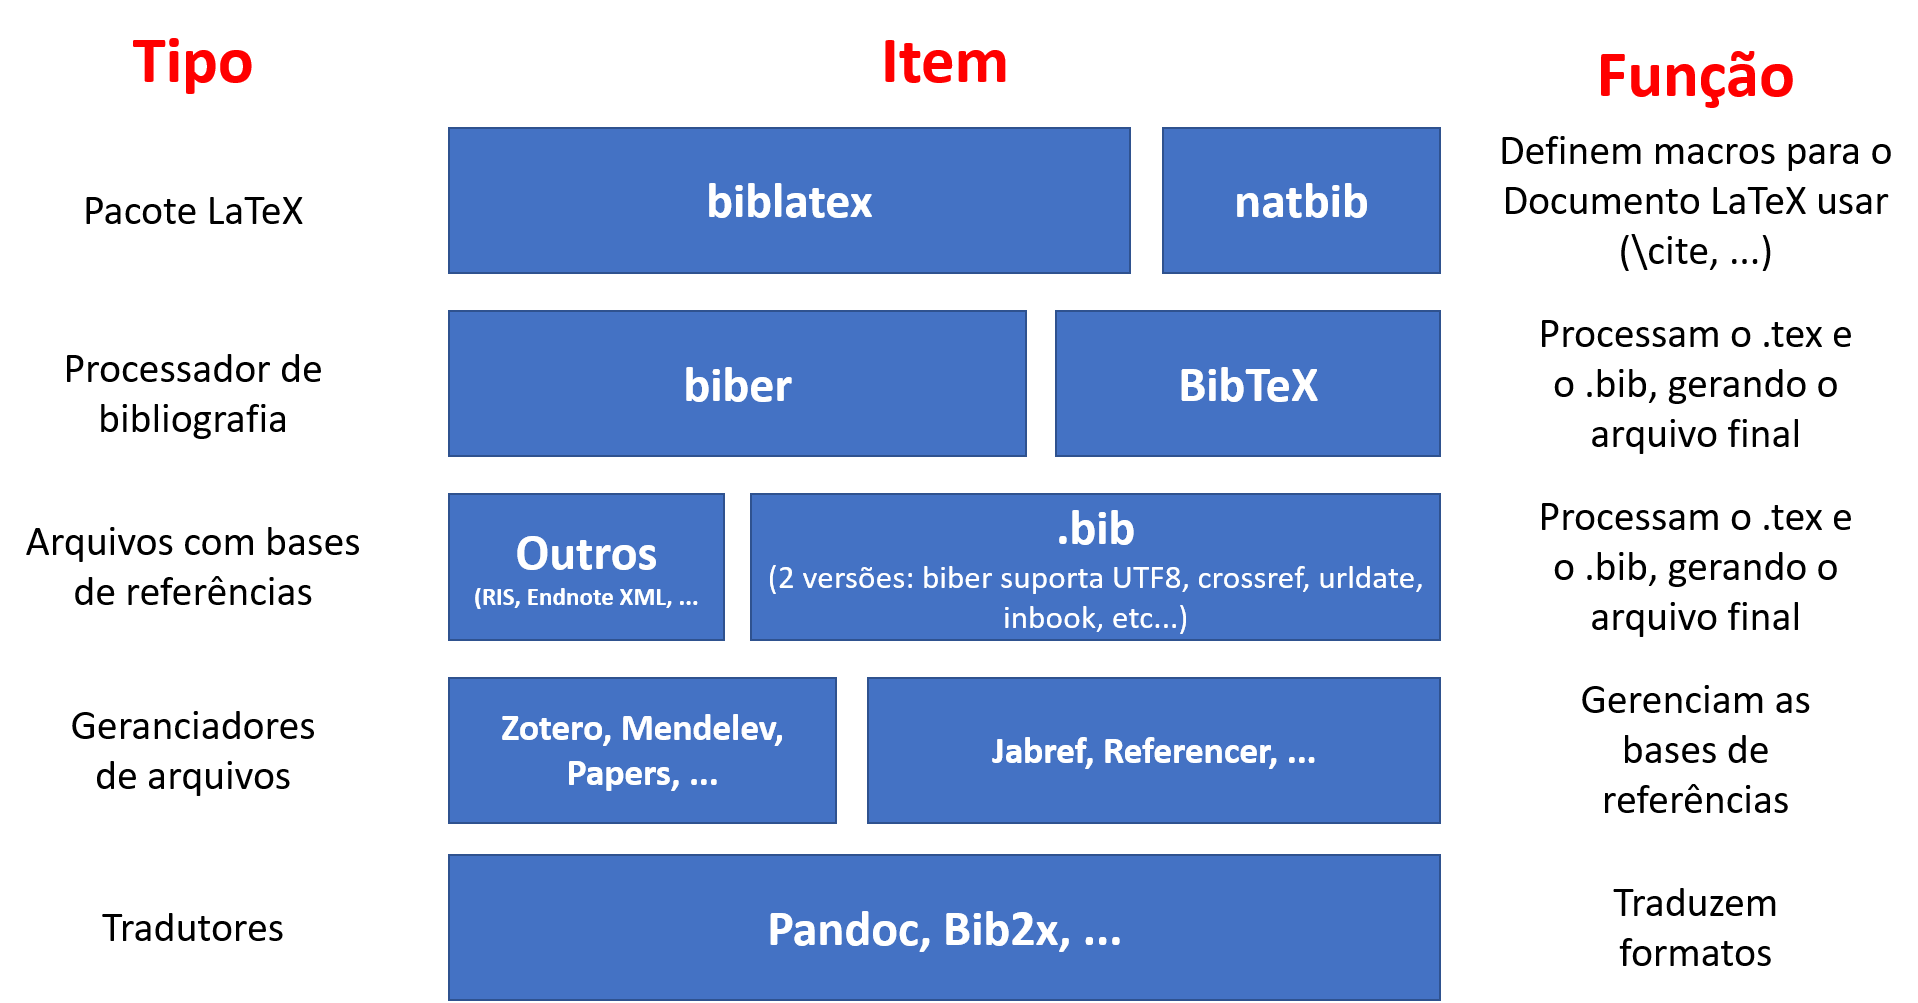
\includegraphics[width=0.9\linewidth]{Images/mundolatexport}
    \caption{O Ecossistema \hologo{BibTeX}\parencite{bibera2012}.}
    \label{fig:mundolatexport}
\end{figure}



A figura \ref{fig:latex-processing-flow2}\footnote{É uma cópia da figura \ref{fig:latex-processing-flow}.} mostra o funcionamento básico quando o biblatex e usado. Um ciclo que usa o natbib pode precisar de mais uma compilação com o processador \LaTeX\  de escolha. Basicamente o processador \LaTeX\   gera um arquivo que contém as informações sobre as citações feitas no documento. Essa informação está no .bcf no caso do biblatex com o \hologo{biber}. Esse arquivo é usado, junto com os vários arquivos .bib contendo as bases de dados de referências utilizadas, para gerar um arquivo .bbl, que contém a bibliografia. Esse arquivo é usado, novamente pelo processador \LaTeX, para gerar o documento final. 


\begin{figure}[hbt]
    \centering
    \includegraphics[width=0.8\linewidth]{"Images/LaTeX processing flow"}
    \caption{O fluxo de processamento (simplificado) do \LaTeX}
    \label{fig:latex-processing-flow2}
\end{figure}

\section{Comparando as Opções}

Como se pode deduzir da figura \ref{fig:mundolatexport}, duas comparações básicas devem ser feitas: dos processadores, biber ou bibtex, e dos pacotes \LaTeX, natbib ou biblatex.

\subsection{natbib vs biblatex}

As duas principais opções de pacotes \LaTeX\    
para referências são o natbib e o biblatex\parencite{biber:2012}:

%%CHECK 2


\begin{outline}
    \1 \textbf{natbib} -- é um pacote antigo e estável, porém ele é  mantido mas não evoluído. 
    \2 Vantagens
    \3 Vários formatos já definidos (arquivos .bst)
    \3 Possui um pacote custom-bib, com o aplicativo makebst, que gera estilos bibliográficos, .bst, iterativamente
    \2 Desvantagens
    \3 Depende do \hologo{BibTeX}, que tem algumas desvantagens.
    \3 .bst é difícil de fazer (linguagem posfixa)
    \3 Orientado para autor-ano e numérico, mas não autor-título, tipo de citação que aparece em outras áreas não tecnológicas
    \3 É fácil pegar a bibliografia gerada e incluir no arquivo .tex, o que algumas editoras pedem.
    \1 \textbf{biblatex} -- ativamente desenvolvido e em evolução, ligado
    ao \textit{backend} mais poderoso \hologo{biber}. Substitui o natbib, e tem pacotes adicionais, como o \lstinline|biblatex-abnt|.
    \2 Vantagens
    \3 Mais campos
    \3 Unicode no arquivo .bib, sem problemas para caracteres de outras línguas que podem aparecer em nomes de autores;
    \3 Usa métodos de \LaTeX\ para controle fino da sua bibliografia;
    \2 Desvantagens
    \3 Algumas revistas podem não aceitar (porque não fizeram o
     \textit{upgrade} de seus estilos).
    \3 Não é fácil pegar a bibliografia criada e inserir no arquivo .tex, o que algumas editora pedem.
\end{outline}


\subsection{\hologo{BibTeX} vs \hologo{biber}}

Os dois principais processadores de referências são o \hologo{BibTeX} e o  \hologo{biber}:
\begin{outline}
    \1 \hologo{BibTeX}
    \2 Se for obrigado, use 
    \2 Estável e debugado
    \2 Problemas com caracteres não padrão 
    \2 Funciona com natbib e biblatex
    \1 \hologo{biber}
    \2 Prefira usar o  biber
    \2 Suporta UTF8!
    \2 .bib file muito mais verificado
    \3 Dá erros novos
    \2 Só funciona com biblatex
\end{outline}



\section{Usando biblatex e biber}

Para usar o biblatex e o \hologo{biber} é necessário:
\begin{itemize}
    \item usar os pacotes csquotes e xpatch
    \item usar o pacote biblatex, escolhendo o backend biber e um estilo
    \item adicionar os arquivos com as bases de referênica
    \item citar os documentos ao longo do artigo
    \item incluir a bibliografia
\end{itemize}
Exemplos de comandos para fazer isso estão na listagem \ref{list:bib1}

\begin{lstlisting}[caption=Exemplo de uso de biblatex,label=list:bib1]
\usepackage{csquotes}
\usepackage{xpatch}
\usepackage[backend=biber,style=numeric]{biblatex}
\addbibresource{references.bib}
...
\cite{biber:2012}
...
\printbibliography
\end{lstlisting}


%\begin{lstlisting}[caption={Controlando a forma de citação com o formato natbib.},label=keyfig:citet]
%\citet{biber:2012} não fala nada sobre isso. 
%Mas \citep{bibera2012} também não. 
%Por isso \citep{biber:2012} não tem erro. 
%\end{lstlisting}

\subsection{Exemplo dos comandos do biblatex}
%\begin{lstlisting}[caption={Exemplo dos comandos do biblatex},label=com:biblatex]
\begin{figure}[hbt]
\centering
\begin{LTXexample}[pos=b]

\autocite{biber:2012}

\cite{biber:2012}

\parencite{biber:2012}

\textcite{biber:2012}

Lorem\footcite{biber:2012}

\fullcite{biber:2012}
\end{LTXexample}
\caption{Exemplo do uso de formas de citações no biblatex}
\label{fig:cite}
\end{figure}
%\end{lstlisting}





\section{Programas Externos}

Vários são os programas externos que podem ser usados
para gerenciar arquivos .bib, entre ele:

\begin{itemize}
    \item JabRef (Java) -- um gerenciador de referências que usa o arquivo .bib como seu formato padrão e pode ser integrado com IDEs \LaTeX;
    \item Referencer (GNOME) -- outro gerenciador de referências, só funciona no GNOME;
    \item BiB2x  -- um processador que transforma do formato .bib para outros, e
    \item Zotero mais Better \hologo{BibTeX} for Zotero -- uma extensão ao Zotero que permite gerar um arquivo .bib contendo as citações feitas em um documento .tex.
\end{itemize}


\subsection{JabRef}
O JabRef, cuja a tela é apresentada na figura \ref{fig:jabref},  é um programa com as seguintes características:
\begin{itemize}
    \item Feito em Java
    \item Open Source
    \item Gerencia vários arquivos .bib em abas
    \item Permite unificar arquivos
    \item Suporte ao biblatex (UTF8,...)
    \item Detecta erros
    \item Busca na web
\end{itemize}


\begin{figure}[hbt]
    \centering
    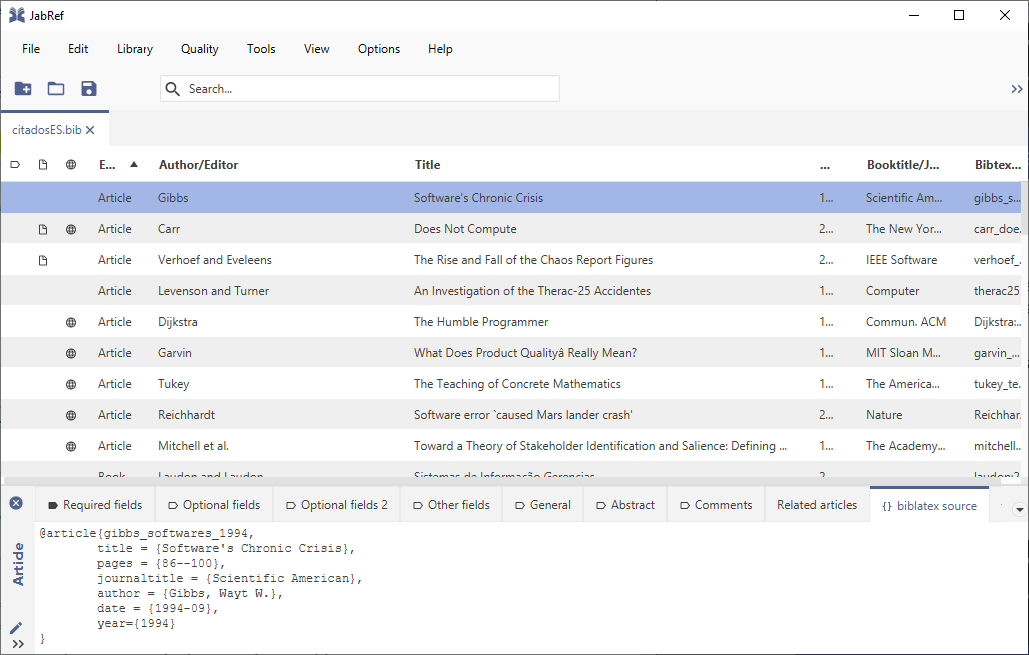
\includegraphics[width=0.7\linewidth]{Images/jabref}
    \caption{Exemplo de tela do Jabref.}
    \label{fig:jabref}
\end{figure}  







